
\section{\label{sec:preliminary}Preliminary Results}
As a preliminary assessment, a constant Young’s modulus can indeed be used with reasonable thicknesses along the chord. The purpose is to provides a strict verification benchmark and this test case serves more for demonstration purposes.
An investigation of the Fluid and structure response to different Re and Young Modulus $\mathcal{E}$ is discussed in the following sections, and each aspect of the FSI will be presented in relation to the findings  at a fixed moderate angle of attack of 15$^{\circ}$.
Differences in the tip deflection (Sec.\ref{sec:deflection}) and fluid-structure response are described in the following sections (Sec.\ref{sec:fluidStrucutreRespnseToYoungAndRey}).

%%%%%%%%%%%%%%% Fluid %%%%%%%%%%%%%%%%%%%%%%%%%%%%%%%%%%%%%%%%%%%%%

%%%%%%%%%%%%%%%%%%%%%%%%%%%%%%%%%%%%%%%%%%%%%%%%%%%%%%%%%%%%%%%%%%%%

\subsection{\label{sec:deflection} Tip deflection}

Here some results of the FSI implementation are illustrated for both Young's modulus 689.5 MPa and 2.5GPa and shown in Figure \ref{fig:history}. The tip deflection history is shown in function of the displacements in the longitudinal direction for the tip control point on the trailing edge.\\

It illustrates the numerical computation of FSI which is performed in two stages.
The standard approach for coupling fluid and structural solvers is to solve the fluid dynamic equations first, then transfer the computed loads to the structural equations.
First the transient fluid flow is computed without coupling the fluid and structure interaction considering the whole airfoil as rigid body. After the flow is developed along the wing, the system is coupled at a coupling time period of t$^*$=0.9s and takes into account the flexible segment of the airfoil.\\
An initial comparison between used Young's modulus $\mathcal{E}$ = 2.5 GPa in literature and  a reduced one E = 689.5 MPa can be done using the preliminary results obtained for a Re= $10^5$ case. \\

In terms of the amount of deflection, the case with $\mathcal{E}$ = 689.5 MPa show a maximum value of deflection 10$\%$ of flexible part (we denote $\mathcal{L}$) (Fig. \ref{fig:deflection689.5MPa}). However, the tip deflection is thought to remain in fluctuation motion. Unlike the previous deformation, and for a Young's modulus $\mathcal{E}$= 2.5GPa, this displacement of the trailing edge tip is deflecting upwards in the same direction of the freestream velocity $\mathcal{U}_\infty$ with a maximum value of deflection 2.2$\%$ of $\mathcal{L}$ (Fig. \ref{fig:deflection2.5GPa}). The results from $\mathcal{E}$= 2.5GPa show that a limited amount of fluctuations and demonstrate a state of slowdown. 

\begin{figure}[hbt!]
\centering
\begin{subfigure}{.4\textwidth}
   \includegraphics[width=3.2in]{Figures/deflection689MPa090.ps}
%   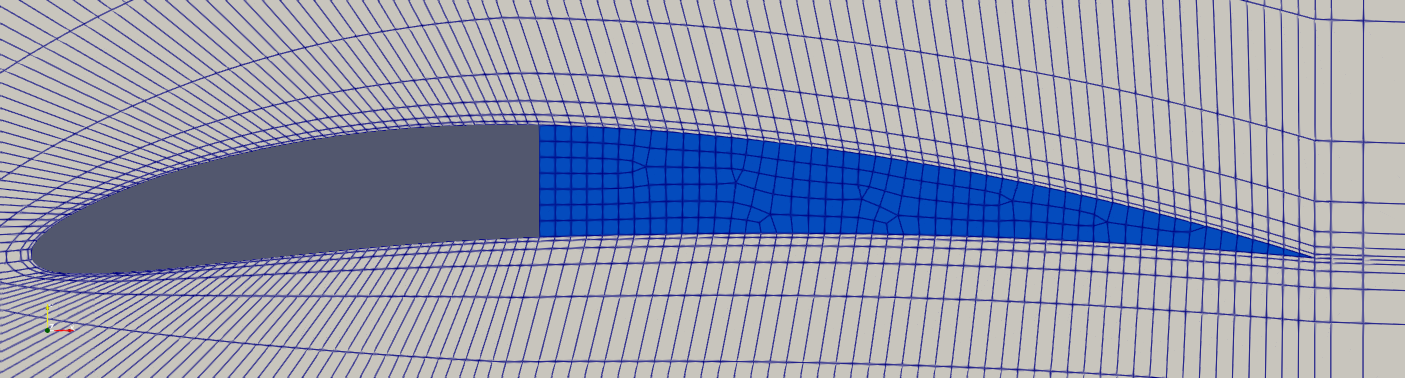
\includegraphics[width=3in]{Figures/mesh solid.png}
  \caption{\label{fig:deflection689.5MPa}}
\label{fig:airfoildesigna}
\end{subfigure}
\begin{subfigure}{.4\textwidth}
   \includegraphics[width=3.2in]{Figures/deflection25GPa10.ps}
%   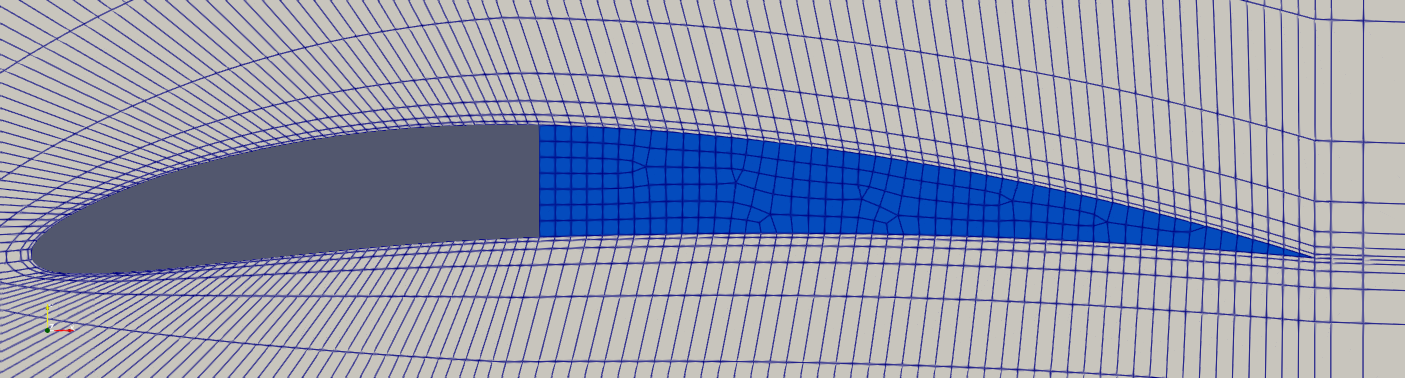
\includegraphics[width=3in]{Figures/mesh solid.png}
  \caption{\label{fig:deflection2.5GPa}}
\label{fig:airfoildesigna}
\end{subfigure}
\caption{\label{fig:history} Tip deflection in y direction at $\mathcal{R}_e$ =100,000; (a) Young modulus $\mathcal{E}$ = 689.5MPa  (b) $\mathcal{E}$ = 2.5GPa }
  \end{figure}

\subsection{\label{sec:fluidStrucutreRespnseToYoungAndRey} Fluid-structure response}
To assess the displacement in the longitudinal direction, the Figure \ref{fig:dispMagni689.5MPa}-\ref{fig:deflection2.5GPa} shows the modal shapes of structural displacement fluctuations for Young modulus $\mathcal{E}$ = 689.5MPa  and $\mathcal{E}$ = 2.5GPa, respectively.The distribution of the displacement over the flexible segment $\mathcal{L}$ grow bigger towards the wing tip owing to large displacements at the tip for both values of $\mathcal{E}$. Though, the lower $\mathcal{E}$ exhibits higher tip deflection. Despite the differences, these displacement distribution provide support that the high $\mathcal{E}$ generates a suddenly increase in deflection. The computed instantaneous velocity colored streamlines are shown in Figure \ref{fig:velocity&Displacement} (left figures) for $\mathcal{E}$ = 689.5MPa  as well as the corresponding displacement magnitude contour of the flexible segment (right figures). A small trailing edge bubble is formed and increases in diameter. These separation bubbles come in a variety of sizes depending on the tip deflection. For $\mathcal{E}$ = 2.5GPa, it is not unexpected to see a small fluctuation of the tip and tends to be stable with the fluid flow over the flexible segment. Therefore the stable state of the tip deflection is highlighted in the Figure \ref{fig:25GPA} and shows it relaxes towards steady-state structure.\\

\begin{figure}[hbt!]
\centering
\begin{subfigure}{.8\textwidth}
    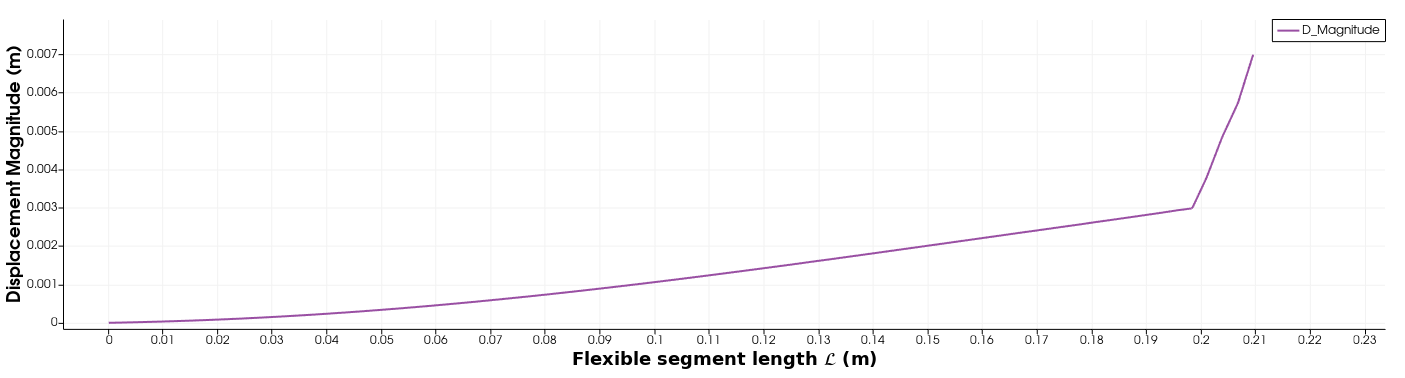
\includegraphics[width=5in]{Figures/DispMAgnitude689MPa.png}
  \caption{\label{fig:dispMagni689.5MPa}}
\end{subfigure}
\begin{subfigure}{.8\textwidth}
    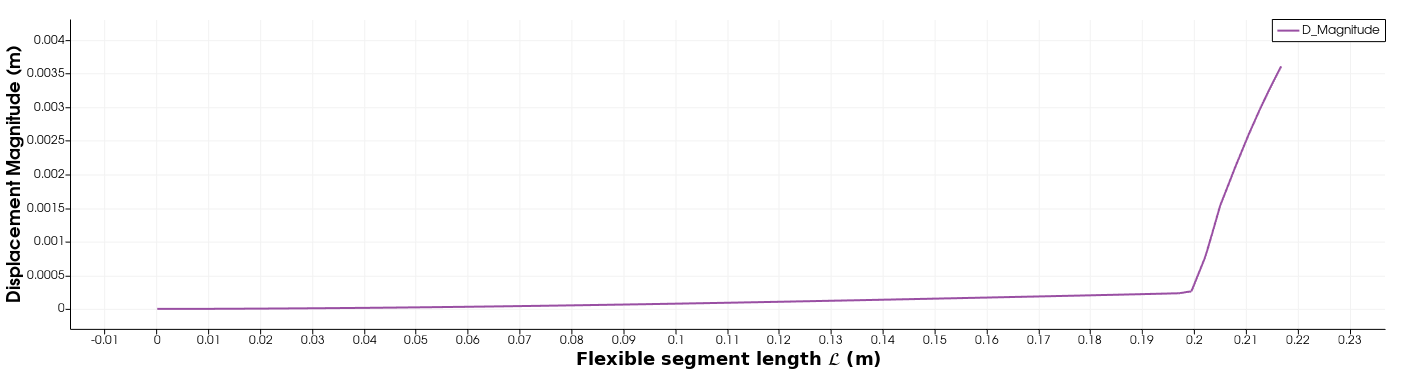
\includegraphics[width=5in]{Figures/DispMAgnitude25GPa.png}
%   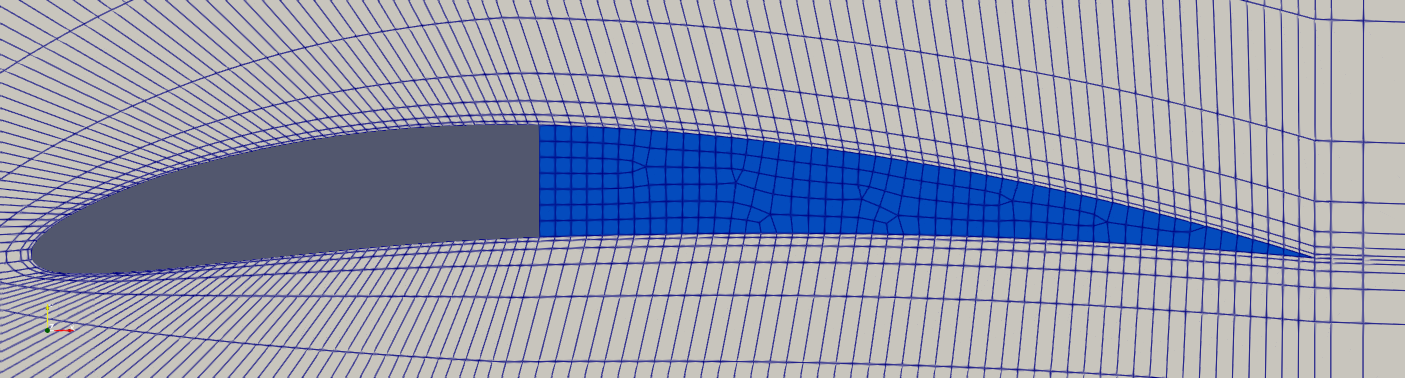
\includegraphics[width=3in]{Figures/mesh solid.png}
  \caption{\label{fig:deflection2.5GPa}}
\end{subfigure}
\caption{\label{fig:displ} Displacement magnitude distrubution at (a) Young modulus $\mathcal{E}$ = 689.5MPa  (b) $\mathcal{E}$ = 2.5GPa }
  \end{figure}

Another goal of deformation control is to keep maximum wing deformation to a minimum in order to avoid damage from large stresses which is critical for control in aeroelastic applications, as it reduces material fatigue caused by vibrations and structural failures caused by high stresses.
The equivalent stress contour over the $\mathcal{L}$ segment and its distubution in chordwise direction are presented Figure \ref{fig:stress} and \ref{fig:stress2.5GPa},respectively. The features learned from the distribution of equivalent stress over the $\mathcal{L}$ segment for $\mathcal{E}$ = 2.5GPa shows promising stress relaxation with Young modulus .

\begin{figure}[hbt!]
  \centering
    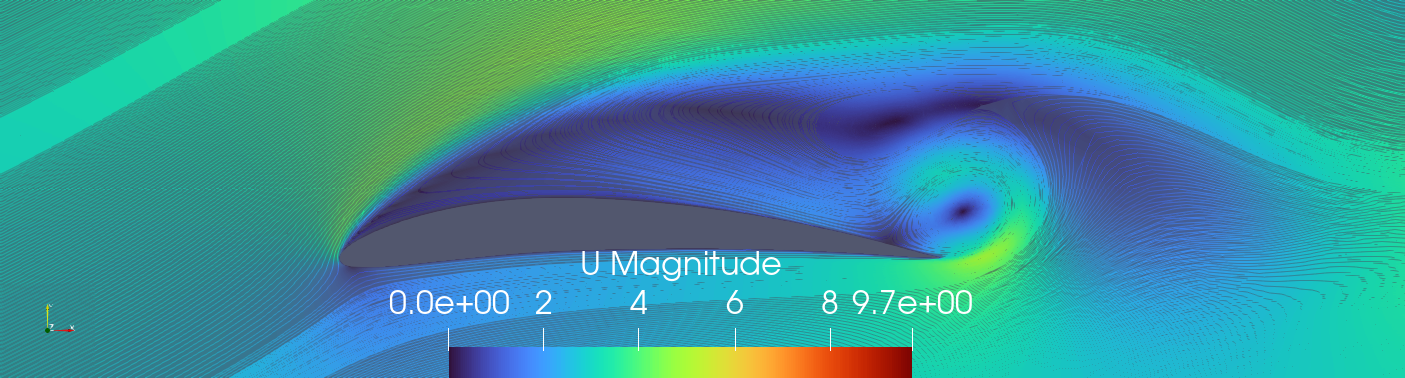
\includegraphics[width=3in]{Figures/streamLines0906Coupling.png}
    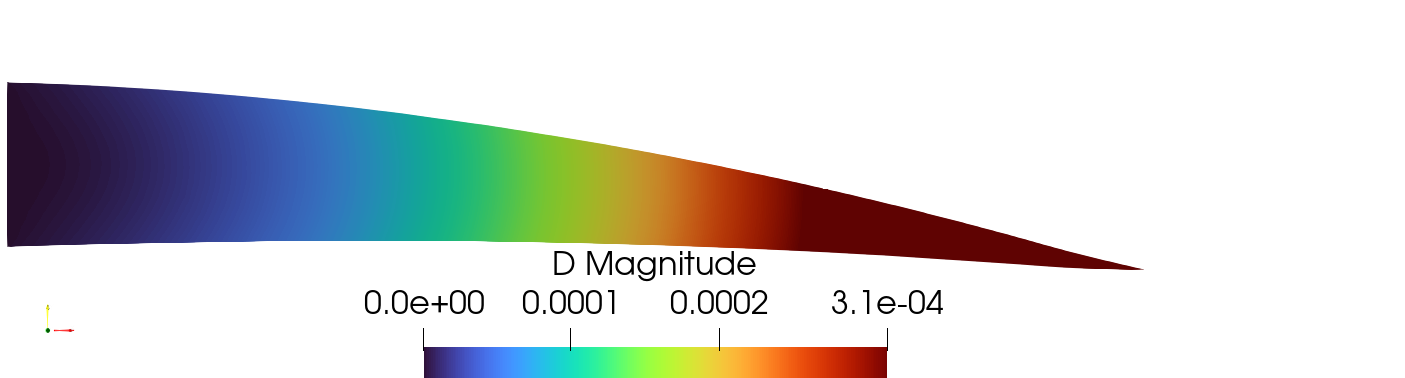
\includegraphics[width=3in]{Figures/DMAgnitude0906Coupling.png}
    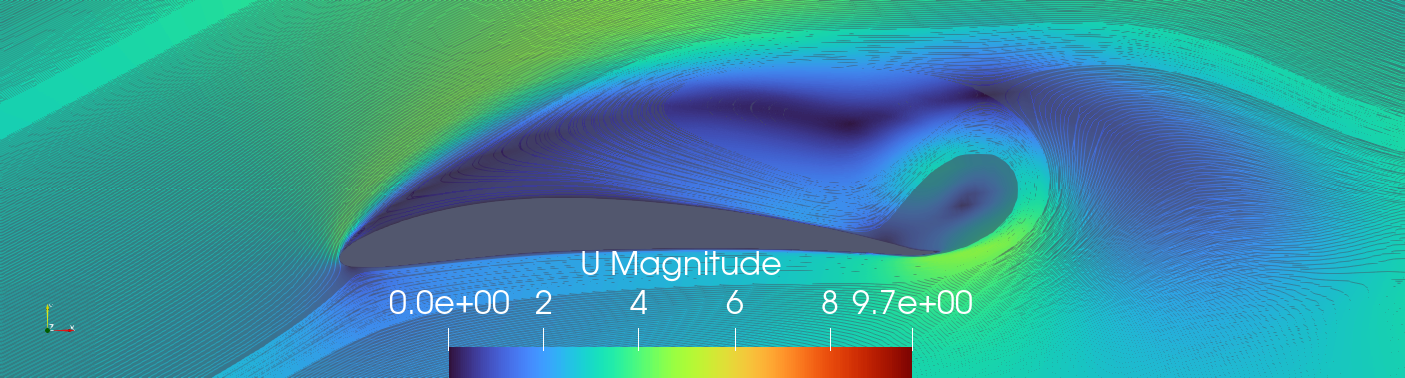
\includegraphics[width=3in]{Figures/streamLines0918Coupling.png}
    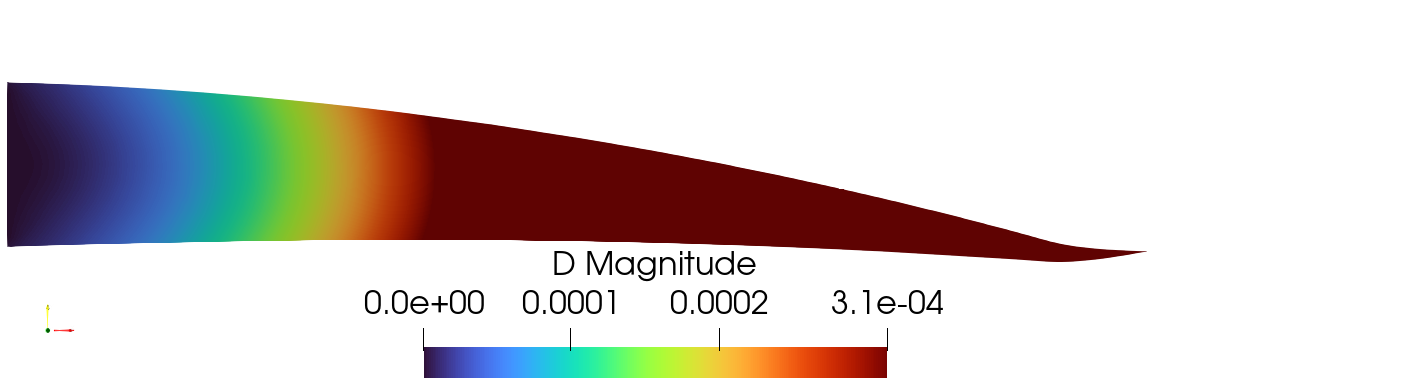
\includegraphics[width=3in]{Figures/DMAgnitude0918Coupling.png}
    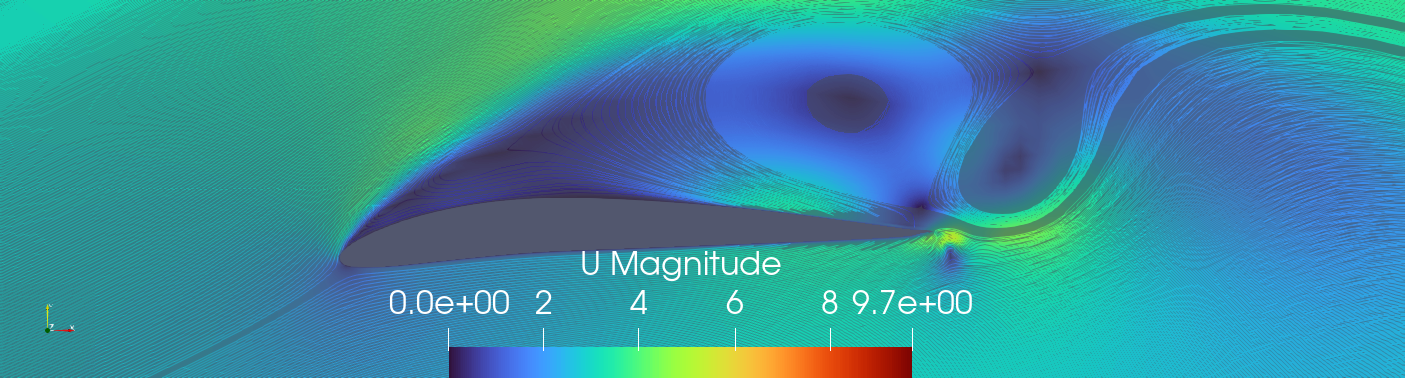
\includegraphics[width=3in]{Figures/streamLines0958Coupling.png}
    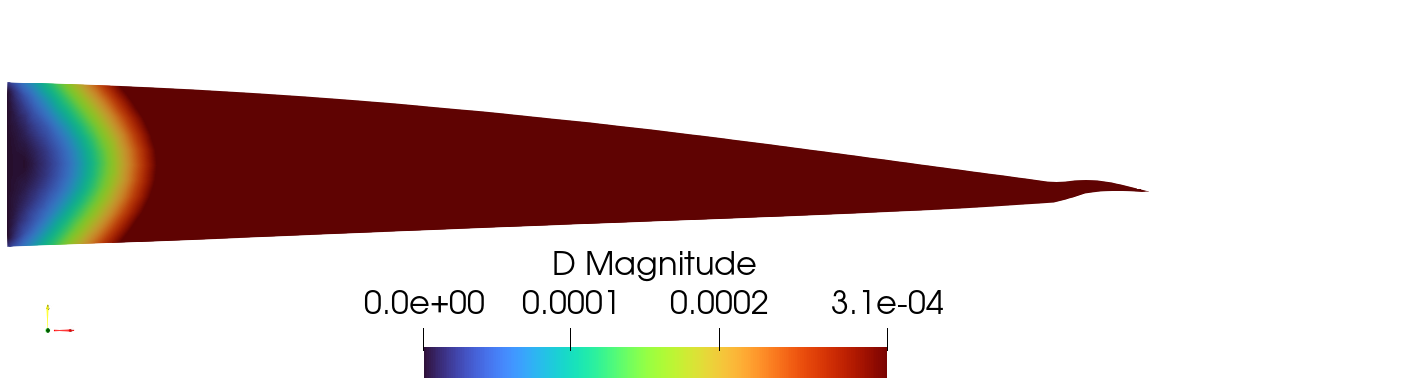
\includegraphics[width=3in]{Figures/DMAgnitude0958Coupling.png}
    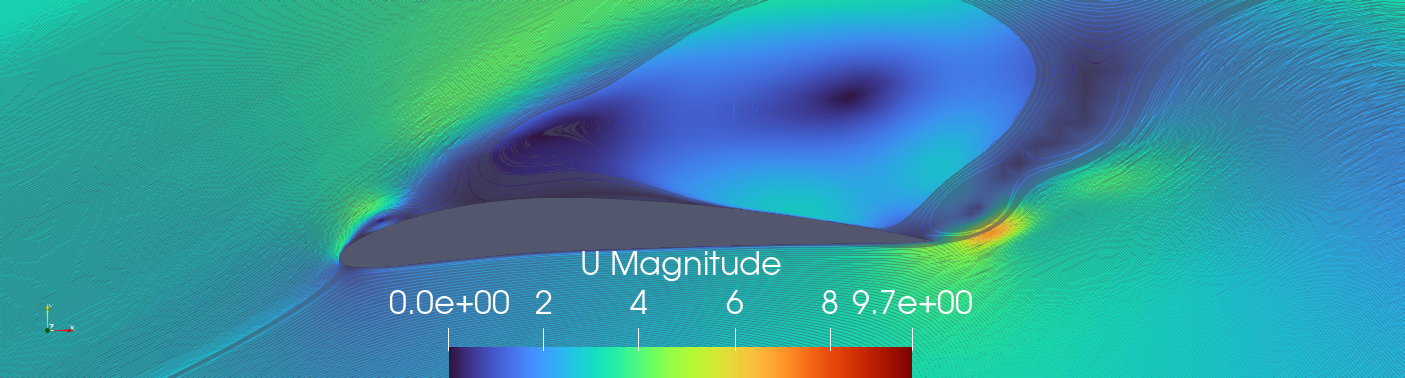
\includegraphics[width=3in]{Figures/streamLines0986Coupling.png}
    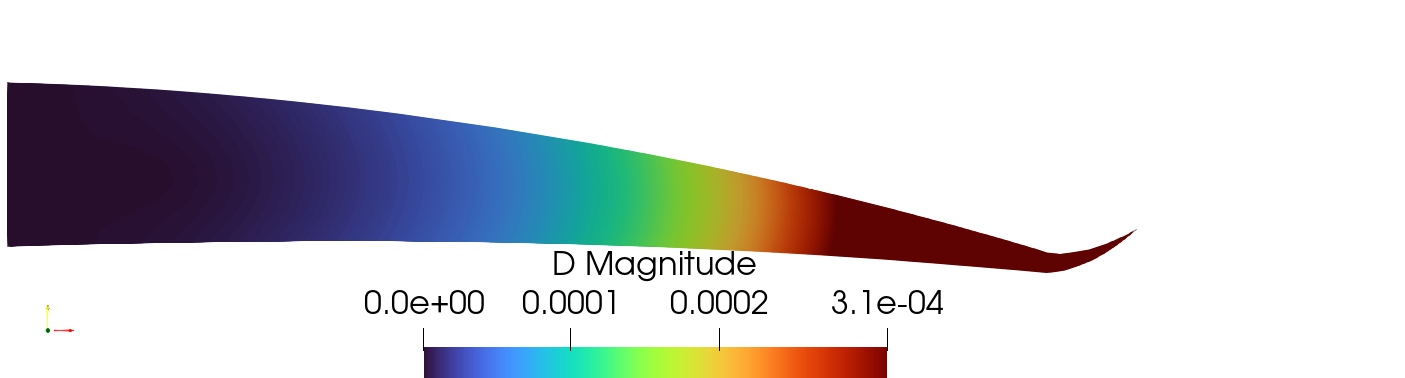
\includegraphics[width=3in]{Figures/DMAgnitude0986Coupling.png}
    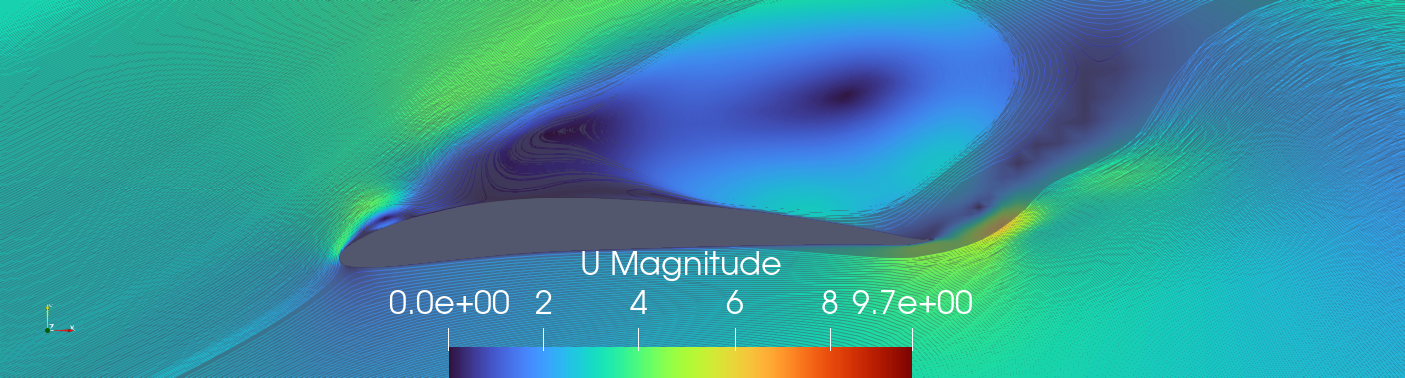
\includegraphics[width=3in]{Figures/streamLines0988Coupling.png}
    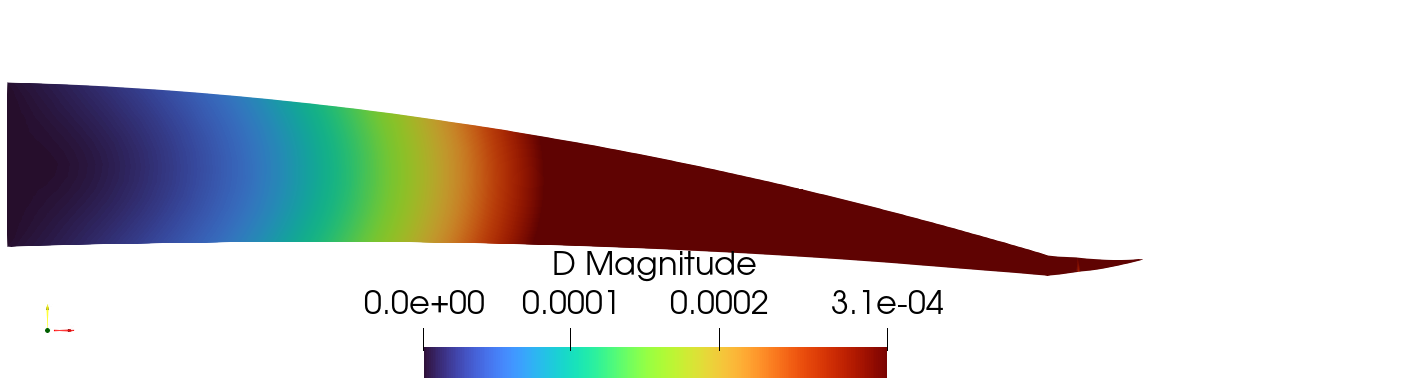
\includegraphics[width=3in]{Figures/DMAgnitude0988Coupling.png}
    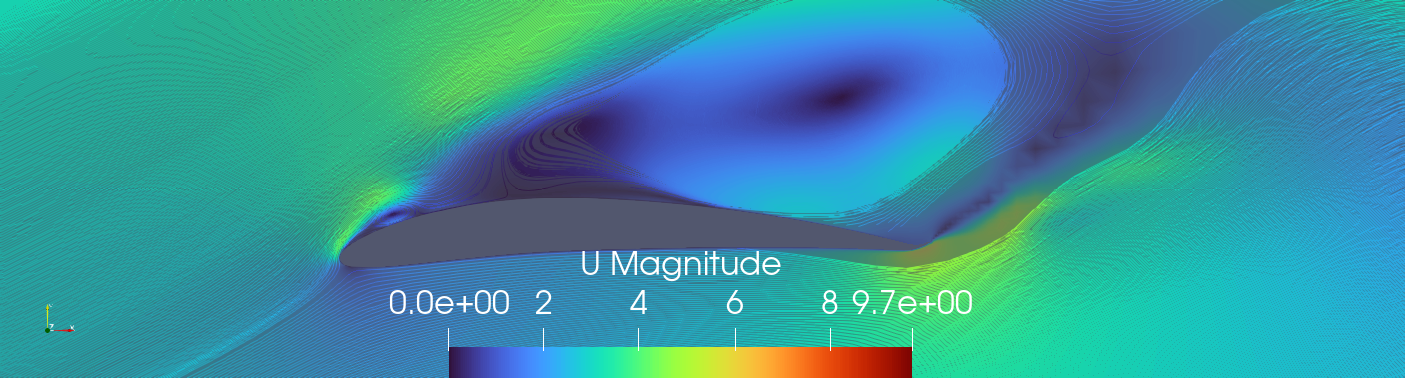
\includegraphics[width=3in]{Figures/streamLines0992Coupling.png}
    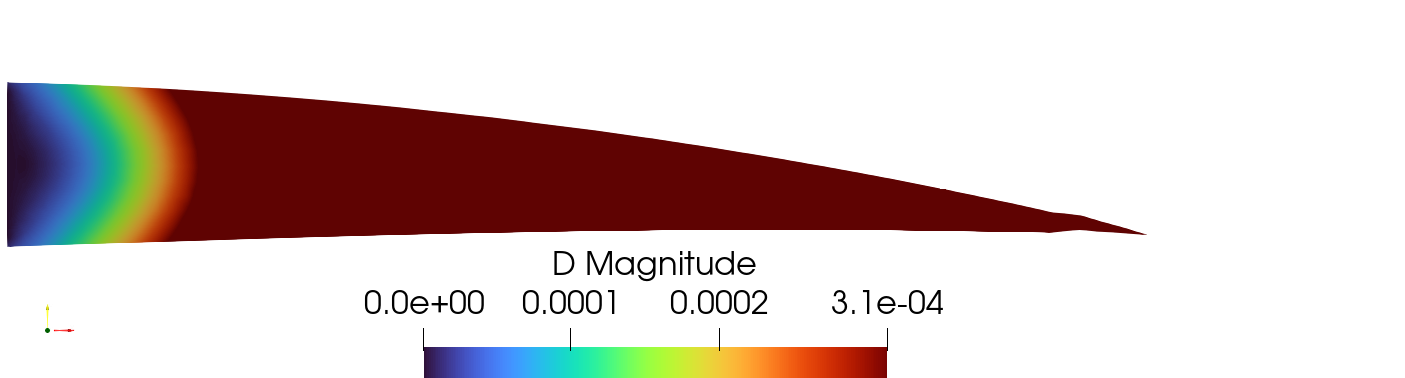
\includegraphics[width=3in]{Figures/DMAgnitude0992Coupling.png}
    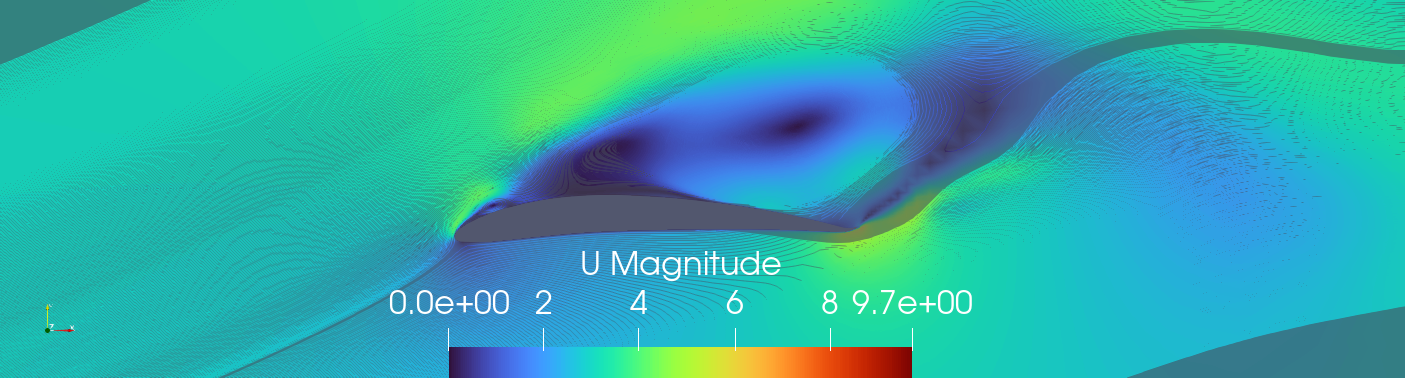
\includegraphics[width=3in]{Figures/streamLines0998Coupling.png}
    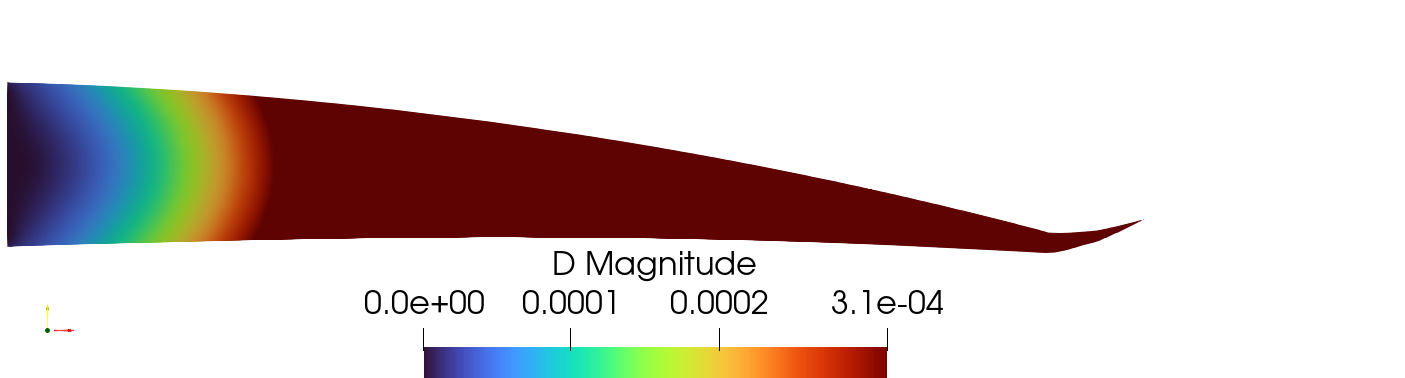
\includegraphics[width=3in]{Figures/DMAgnitude0998Coupling.png}
  \caption{\label{fig:velocity&Displacement} Velocity colored flowfiel streamlines (right) displacement contours (left) $\mathcal{R}_e$ =100,000 $\mathcal{E}$= 689.5MPa}
\end{figure}

\begin{figure}[hbt!]
  \centering
    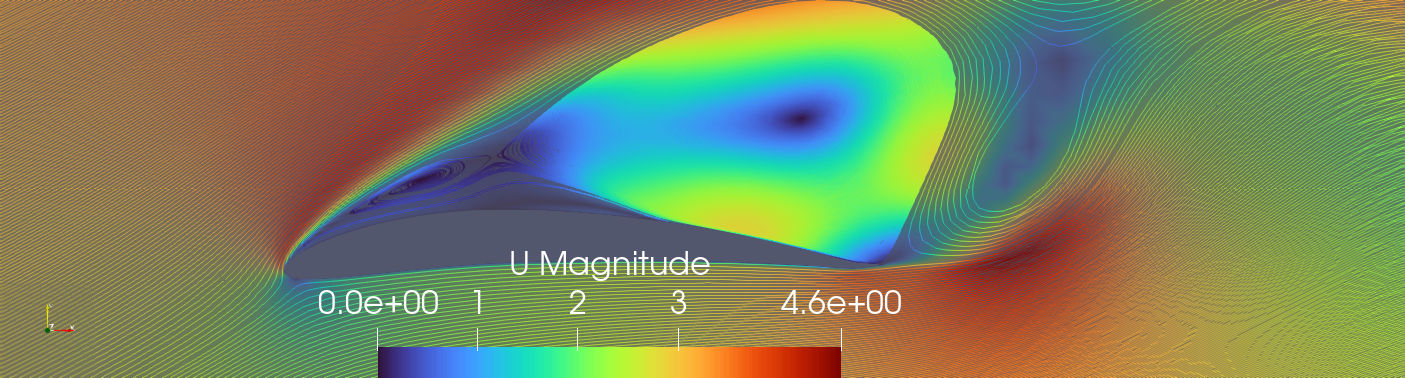
\includegraphics[width=3in]{Figures/streamLines25GPACoupling.png}
    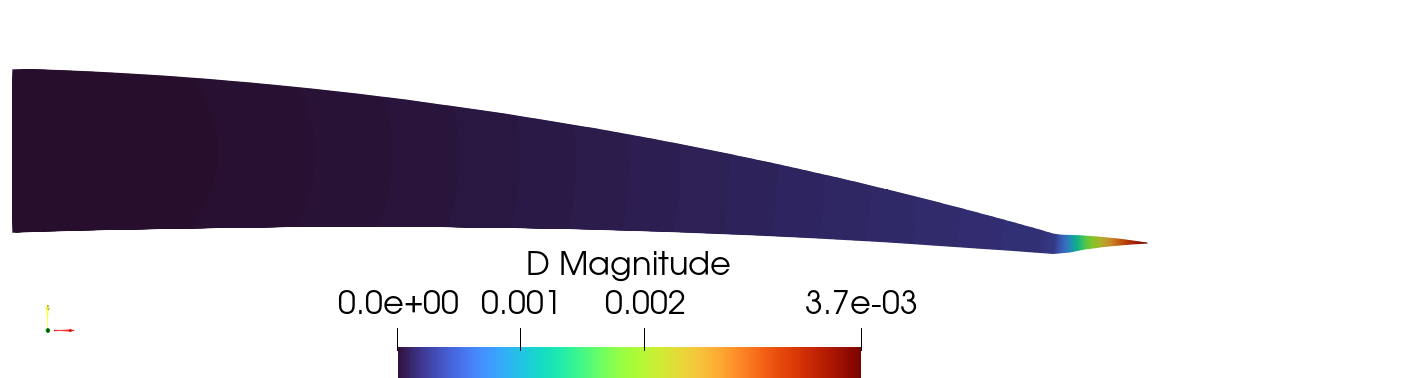
\includegraphics[width=3in]{Figures/DMAgnitude25GPaCoupling.png}
  \caption{\label{fig:25GPA} Velocity colored flowfiel streamlines (right) displacement contours (left) $\mathcal{R}_e$ =100,000 $\mathcal{E}$= 2.5GPa}
\end{figure}

\begin{figure}[hbt!]
\centering
\begin{subfigure}{.6\textwidth}
   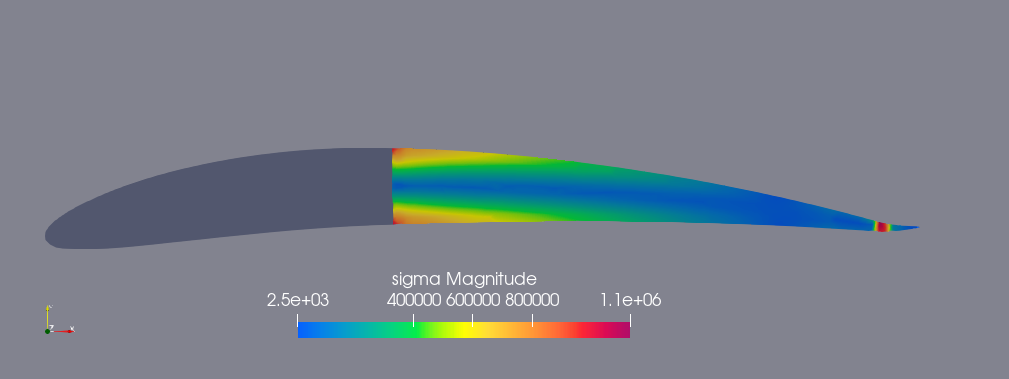
\includegraphics[width=3in]{Figures/sigma.png}
     \caption{\label{fig:stress} Equivalent stress contour over the flexible segment}
\end{subfigure}
\begin{subfigure}{.8\textwidth}
    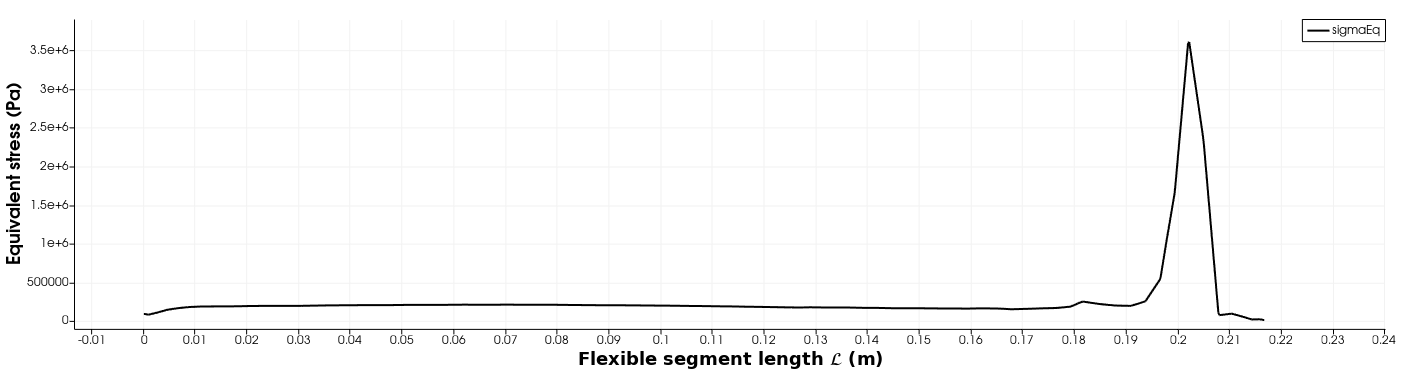
\includegraphics[width=5in]{Figures/equivalent stress.png}
%   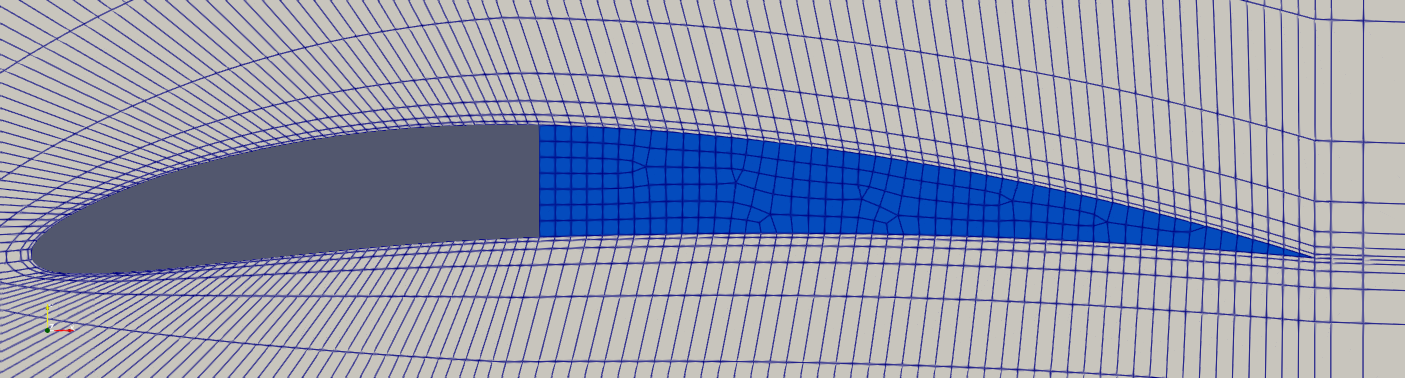
\includegraphics[width=3in]{Figures/mesh solid.png}
  \caption{Chordwise equivalent stress distribution\label{fig:stress2.5GPa}}
\end{subfigure}
\caption{\label{fig:displ} Stress analysis for $\mathcal{E}$ = 2.5GPa }
  \end{figure}







